\documentclass{article}
\usepackage{polski}
\usepackage[utf8]{inputenc}
\usepackage{natbib}
\usepackage{graphicx}
\usepackage{xcolor}
\usepackage{mathtools}
\usepackage{amssymb}
\usepackage[makeroom]{cancel}
\usepackage{hyperref}
\newcommand{\norm}[1]{\left\lVert#1\right\rVert}

\title{Sprawozdanie 2}
\author{Jan Bronicki 249011}
\date{}


\begin{document}

\maketitle



\section{Cel ćwiczenia}
Zapoznanie się z działaniem tranzystorów NPN oraz PNP.

\section{0-10V}
\subsection{$U(V)$}

Dzielnik napięcia z rezystorami $R_{2}$ oraz $R_{5}$, jest potencjometreem $10k\Omega$ sterowany do 99\%:

$$
    U_{wy} = U_{we} \cdot \frac{R_{2}+R_{5}}{R_{1}+R_{2}+R_{5}}
$$
$$
    10V = 24V\cdot \frac{10\Omega}{R_{1}+10\Omega}, R_{1}=14\Omega
$$

Pobierane jest $20mA$, tak więc opór to:

$$
    R_{4} = \frac{10V}{20mA}
$$

Rezystor $R_{3}=470\Omega$ stabilizuje wzmacniacz.

\begin{figure}[h!]
    \centering
    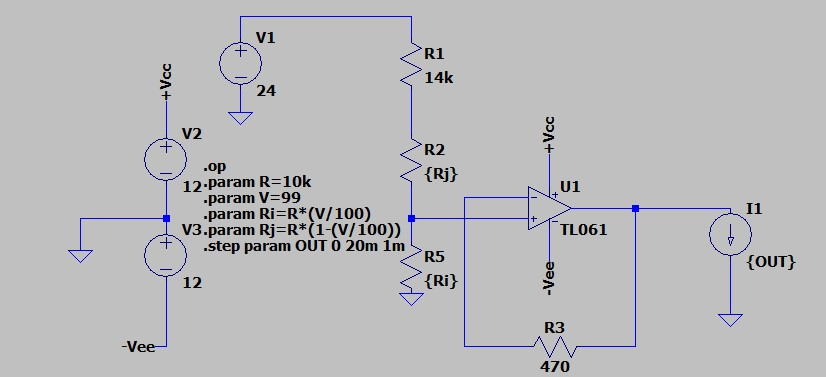
\includegraphics[scale=0.5]{rys1_model.jpg}
\end{figure}

\newpage

\begin{figure}[h!]
    \centering
    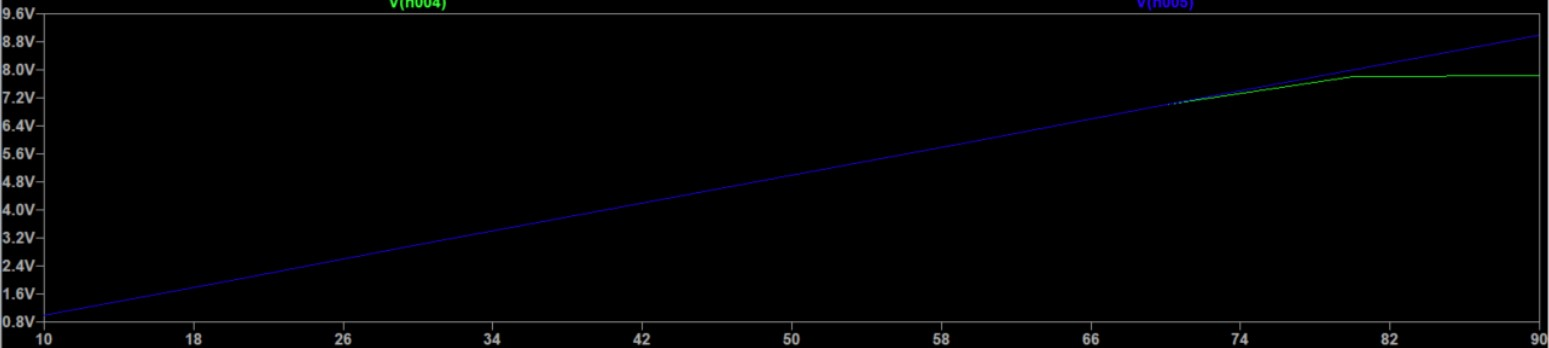
\includegraphics[scale=0.35]{rys1_wykres.jpg}
\end{figure}

Wzmacniacz stabilizuje się na około $7.2V$.


\subsection{$U(R)$}

Napięcie stabilizuje sisę przy $R_{ob} > 620 \Omega$:

$$
    I_{wy} = \frac{U_{wy}}{R_{ob}}
$$

$$
    I_{wy} = \frac{10V}{620\Omega}\approx 16mA
$$


\subsection{$U(I)$}

Układ jest w stanie podać maksymalne natężenie około 16mA, w przybliżeniu zgodne z obliczeniami.

\begin{figure}[h!]
    \centering
    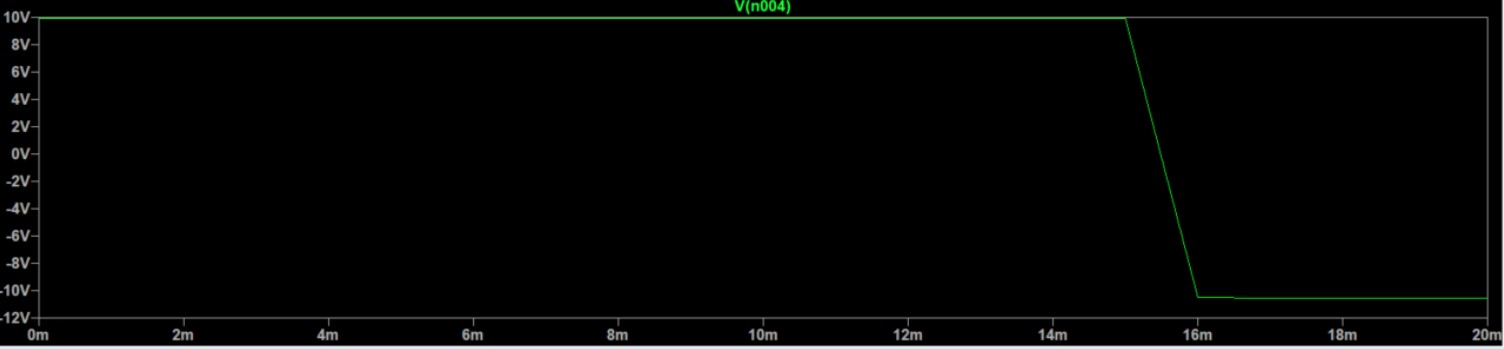
\includegraphics[scale=0.35]{rys2_wykres.jpg}
\end{figure}
\newpage
\begin{figure}[h!]
    \centering
    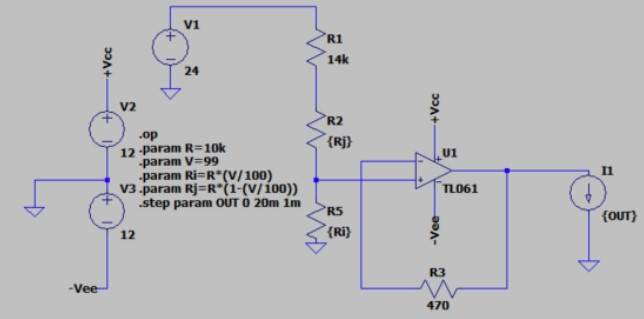
\includegraphics{rys2_model.jpg}
\end{figure}

\newpage

\section{NPN i PNP}

\begin{figure}[h!]
    \centering
    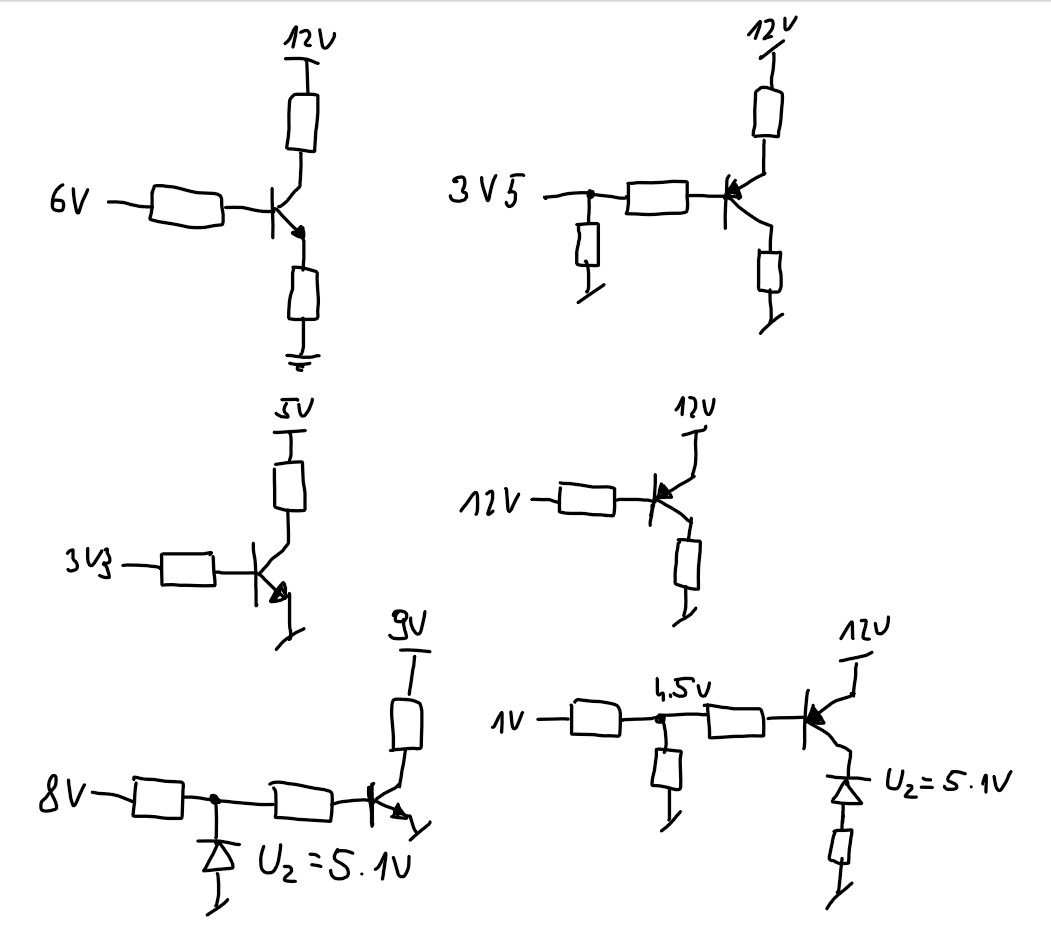
\includegraphics[scale=0.6]{rysunek.jpg}
\end{figure}


\newpage

\subsection{a)}

$U_{ce} = 0.1V, \ U_{be} = 0.6V, \ \beta = 100, \ I_{b} = 1mA, \ R_{3} = 10\Omega$\\
$I_{c}\beta \cdot I_{b}  100mA$\\
$I_{c}+I_{b}=101mA$\\
$U_{R_{3}} = R_{3}\cdot I_{c} = 1.01V$

$$
    R_{1}=\frac{6V-U_{R_{3}}-0.6V}{I_{b}}=\frac{6V-1.01V-0.6V}{0.001A}=4390\Omega
$$

$$
    R_{2}=\frac{12V-U_{R_{3}}-0.1V}{I_{c}}=\frac{12V-1.01V-0.1V}{0.1A}=4390\Omega
$$

\begin{figure}[h!]
    \centering
    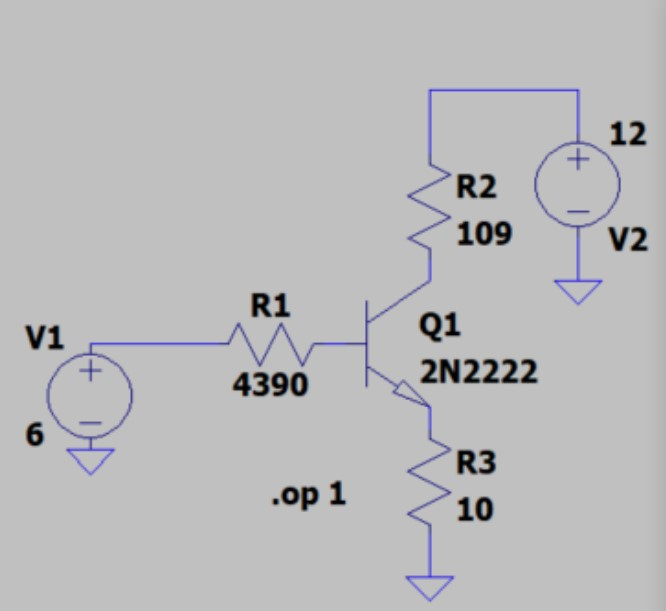
\includegraphics[scale=0.5]{rys3_model.jpg}
\end{figure}


\begin{figure}
    \centering
    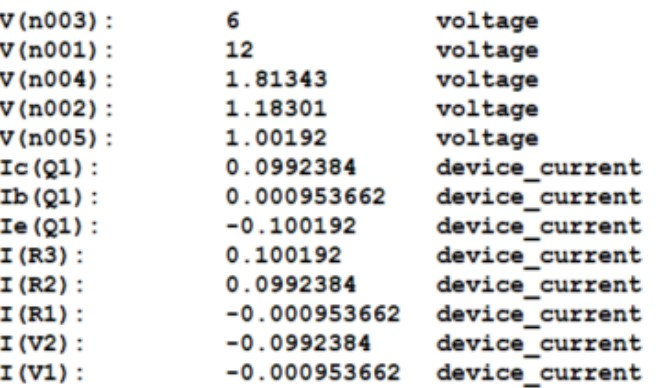
\includegraphics[scale=0.35]{rys3_num.jpg}
\end{figure}

\newpage


\subsection{b)}

$U_{ce} = 0.1V, \ U_{bc} = 0.6V, \ \beta = 100, \ I_{b} = 1mA$\\
$I_{c}=\beta \cdot I_{b} = 100 mA$\\
$I_{e} = I_{c} + I_{b} = 101mA$

$$
    R_{1}=\frac{3.3V-0.6V}{I_{b}}=\frac{2.7V}{0.001A}=22700\Omega
$$

$$
    R_{2}=\frac{5V-0.1V}{I_{c}}=\frac{4.9V}{0.1A}=49\Omega
$$

\begin{figure}[h!]
    \centering
    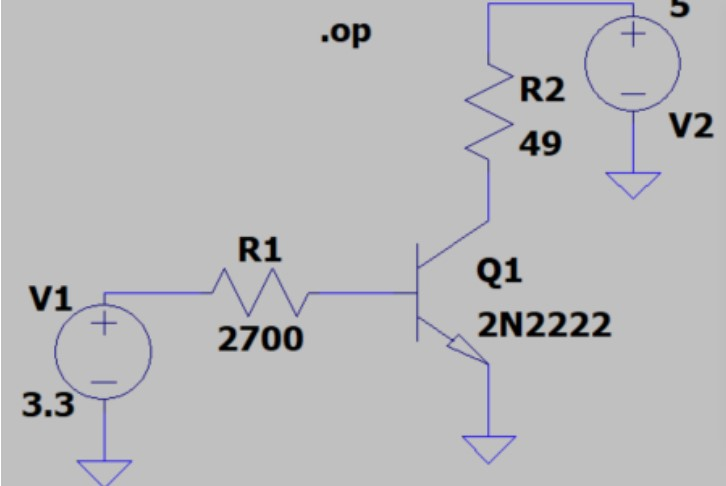
\includegraphics[scale=0.35]{rys4_model.jpg}
\end{figure}

\begin{figure}[h!]
    \centering
    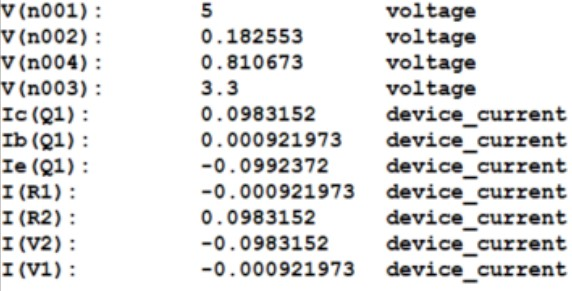
\includegraphics[scale=0.5]{rys4_num.jpg}
\end{figure}

\newpage

\subsection{c)}

$\beta = 100, \ I_{b} = 1mA$\\
$I_{c}=\beta \cdot I_{b} = 100mA$\\
$I_{e}=I_{c}+I_{b}=101mA$

$$
    R_{1} = \frac{U_{R_{1}}}{I_{b}}=\frac{2.9V}{0.001A}=2900\Omega
$$

$$
    R_{2} = \frac{5.1V-0.6V}{I_{b}}=4500\Omega
$$

$$
    R_{3} = \frac{9V-0.2V}{I_{c}}=88\Omega
$$

\begin{figure}[h!]
    \centering
    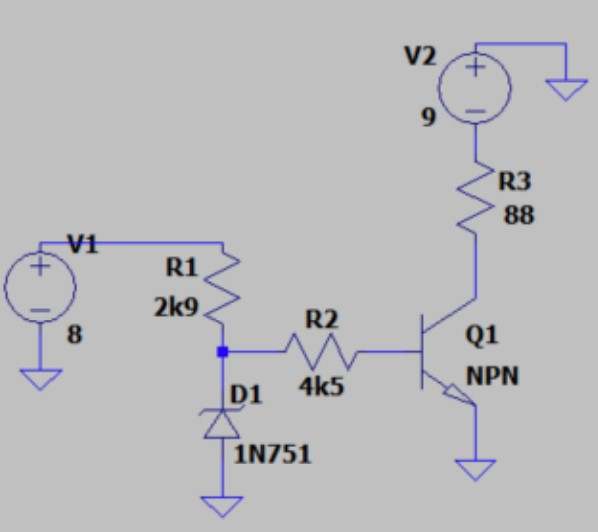
\includegraphics[scale=0.35]{rys5_model.jpg}
\end{figure}


\begin{figure}[h!]
    \centering
    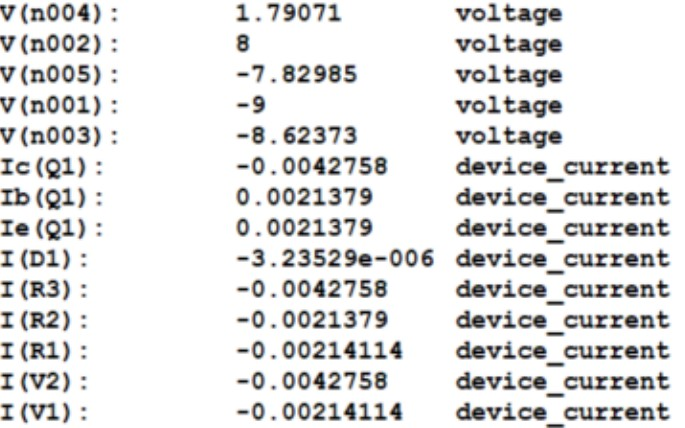
\includegraphics[scale=0.5]{rys5_num.jpg}
\end{figure}

\newpage

\subsection{d)}

$U_{ce}=0.1V, \ U_{be}=-0.6V, \ \beta = 100, \ I_{b} = 2mA, \ R_{4} = 20\Omega$\\
$I_{c}\beta \cdot I_{b} = 200mA$\\
$I_{e} I_{c} + I_{b} = 202mA$\\
$U_{R_{4}} = R_{4} \cdot I_{e}=4.04V$

$$
    R_{3} = \frac{12V-0.1V-U_{R_{4}}}{I_{c}}\approx 39\Omega
$$

$$
    R_{2} = \frac{12V - 3.5V -0.6V -U_{R_{3}}}{I_{b}}=20\Omega
$$

\begin{figure}[h!]
    \centering
    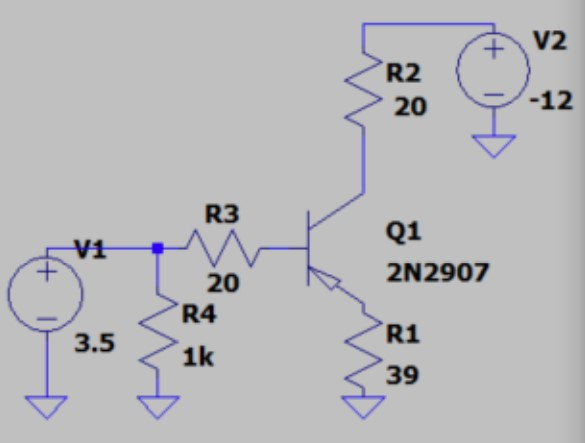
\includegraphics[scale=0.35]{rys6_model.jpg}
\end{figure}

\begin{figure}[h!]
    \centering
    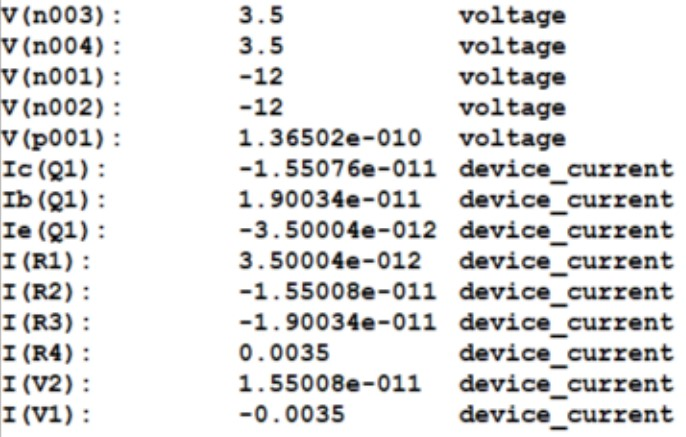
\includegraphics[scale=0.4]{rys6_num.jpg}
\end{figure}

\subsection{e)}
Pomiędzy emiterem a bazą nie będzie prądu, taki układ nie zadziała.

\newpage

\subsection{f)}

$U_{ce} = 0.1V, \ U_{be} = -0.6V, \ \beta = 100, \ I_{b} = 2mA$\\
$I_{c}=\beta \cdot I_{b} = 200mA$\\
$I_{e}=I_{c}+I_{b}=202mA$

$$
    R_{3} = \frac{12V-4.5V-0.6V}{I_{b}}=3450\Omega
$$

$R_{2}$ liczymy z dzielnika napięcia:

$$
    4.5V = \frac{R_{2}}{R_{2}+R_{3}}\cdot (12V-0.6V), \ R_{2} = 2300\Omega
$$

$$
    R_{4} = \frac{12Vv-5.1V-0.1V}{I_{c}}\approx 34\Omega
$$

$$
    R_{2}=\frac{3.5V}{I_{b}}2250\Omega
$$

\begin{figure}[h!]
    \centering
    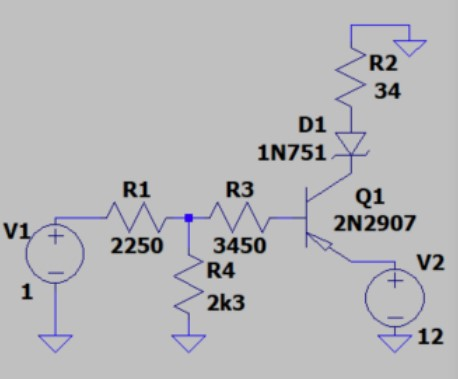
\includegraphics[scale=0.35]{rys7_model.jpg}
\end{figure}


\begin{figure}[h!]
    \centering
    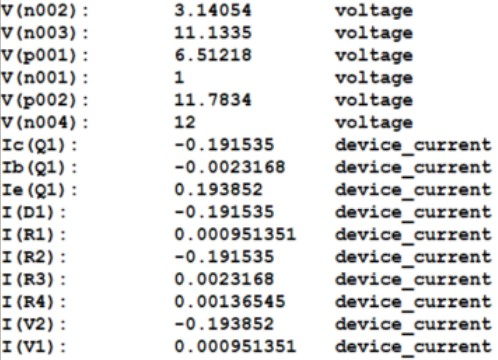
\includegraphics[scale=0.4]{rys7_num.jpg}
\end{figure}





\end{document}
